%!TEX root = project.tex

\chapter*{About this project}
\paragraph{Abstract}
Social media today plays an expanding significant role in society, the information technology industry and the field of computer science. The use of social media is a hot-topic for many organisations, with the aim to identify approaches in which companies can use applications to increase profits and grow product awareness. On a day-to-day basis, users from across the globe are becoming increasingly frustrated, wasting valuable time, scrolling through irrelevant content while companies are wasting money advertising to users outside their market.  In order to achieve the optimal benefits from social media, for both users and businesses, the development of these technologies require approaches that focus on specific human interests and values.

\paragraph{}
This project aims to deliver a solution by developing a platform with the goal of delivering a social experience that targets a specific user base. As the authors are in the field of computer science the focus of the content will be to appeal to the tech savy user. The proposed solution will be a web application that will offer a unique online community to users and businesses interested in technology. 

\paragraph{Authors}
This project was developed as a 15 credit project by Kevin Barry and Cian Gannon, final year students of Software Development at Galway Mayo Institute of Technology.

\paragraph{Acknowledgements}
The authors of this project would like to acknowledge and thank the project supervisors Martin Keniron and Dr. John Healy of GMIT for offering their time and advice throughout this project.
\chapter{Introduction}
During our first three years in GMIT (Galway Mayo Institute of Technology) we were taught a broad range of topics from hardware to software. This was done to get us ready for whatever facet we chose. As part of this project is to show what we learned and put it into practice.

In late 2018, in the first semester of our fourth year, we were told we would be doing a group project over the two semesters. So in October 2018 Kevin Barry and Cian Gannon decided to form a group and started brainstorming ideas in order to start work early. Bringing those ideas to our project supervisors and getting their feedback on our idea we were able to form the idea for our final year project. With input from supervisors and using our own ideas, we were able to move forward with the technologies we would use as our foundation. This was an extremely important decision for us as we wanted to pick relevant technologies and keep the scope within the scope of the level 8 course. 

In our first week of the first year, our student union representatives created a group page on Facebook. This was something which kept everyone in the course in contact with one another outside of college hours. Social media has rapidly expanded in the last ten years, where it's now quite hard to find someone who doesn't have some sort of social media account on one of the numerous platforms. Our world has become ever increasingly dependent on social media and the features it brings.

Looking at social media and how reliant our world has become on it, we wanted to understand it better and have a stronger grasp on the underlying technologies.

\section{Project Objectives} \label{objectives}
As mentioned above, our main goals for this project were to increase our understanding of how social media sites operate, the technologies used to make them and by changing how social media is designed by focusing at a specific target group.

This project is divided into two parts, the research-based dissertation and the applied project. We will be discussing the project in terms of the research behind it and the technologies used to build it. For this reason we split the objectives into dissertation or applied project based. We defined the objectives at a high level allowing us to break each objective into smaller tasks for development.

The objectives set out for the dissertation 
\paragraph{Dissertation}
\begin{itemize}
\item \textit{\textbf{Introduce the concept of the project}}. We will provide the reader with an introduction that describes the concept of the project, detailing its inspiration and goals.
\item \textit{\textbf{Provide an understanding of social media}}. Through extensive research we will examine and outline the concept of social media. We will investigate a vast variety of topics ranging from how social media began, how it became what it is today and what we must do to stay relevant in the modern world.
\item \textit{\textbf{Provide an understanding of web technologies}}. To date, the vast number of technologies available for web development is expanding at a rapid rate. Exploring a range of different technologies we will discuss the pros and cons and give an insight into why we felt our final decision was most suitable for our project..
\item \textit{\textbf{Describe the development of the applied project}}. This dissertation aims to give the reader a comprehensive guide to the development process from the first steps of initial research to the end product. We will examine the approach of the team to the applied project, including methodologies and technologies used along with the design and evaluation of the system. To conclude we will evaluate the project and discuss any issues that occurred, how they were solved and what we would do differently in future development.
\end{itemize}
 
 \paragraph{Applied Project}
\begin{itemize}
\item \textit{\textbf{Produce a simple, easy to use web application}}. The project will implement numerous of complex algorithms with a sophisticated API server and database at the back end. The final product must hide all the complexities from the user with a functional and appealing front. Regardless of the users technical abilities, the web application will be simple to use and navigate.
\item \textit{\textbf{Deliver a social platform for tech savvy people that differs from the norm}}. Changing the way social media applications are generally developed, we will take a different approach and aim to deliver a solution by developing a platform with end goal of delivering a social experience that targets a specific user base. The final application will provide an immerse online community where like minded people can connect, share posts and interact with each other by commenting and giving feedback.
\item \textit{\textbf{Dive into new web technologies}}. For the purpose of expanding the teams knowledge portfolio and skill-set the development will be conducted using new technologies that we previously have not explored. Maximising the learning outcomes of the module by implementing modern practices to result in a streamlined up-to-date application.
\item \textit{\textbf{Complete the project collaborating as a team using an efficient and effective approach}}. The project will be developed as a collaborative effort. Using appropriate tools, methodologies and industry standards available to us, the project will be developed with the aim of simulating real industry experience. With the intention of maximizing efficiency and effectiveness, we will work closely swapping ideas, solving issues and reviewing performance to produce the optimal outcome.
\end{itemize}


\section{Metrics for success or failure} \label{metrics}
In order to create the application in a controlled and easy to manage progress in the early stages of this project it was crucial that we outlined the metrics for success or failure. Doing so, enabled us to keep on track with the core focus of what we were attempting to achieve. The metrics we defined related closely to the the objectives outlined in \ref{objectives}. The simplified list of metrics for success from both a dissertation and web application is as follow:
\begin{itemize}
  \item \textit{A concise, yet comprehensive dissertation which can be understood by anyone regardless of the initial knowledge of the technologies implemented.} To measure this, as each section of the dissertation was roughly drafted up, we released sections to friends and fellow students to read. We would then process their feedback and make alterations were required.  
  \item \textit{A Simple, easy to use, functional web application}. To measure this we followed the same steps as above, releasing beta versions to friends of different technological abilities, allowing us to receive feedback both from a technical and non technical perspective.
  \item \textit{A social platform that actually develops an online community}.To measure the effectiveness of the application from a social point of view.We kept a log of the user activities while monitoring the site. Thus enabling us to at certain time points be able to see users following more users and interacting with a larger reach.
  \item \textit{Teamwork Collaboration} We felt from a project management perspective and by researching the importance of a good team in industry, that we would measure the success of the team. With each weekly team meeting we would take time to reflect on how we resolved issues and while looking at the strengths and weaknesses of our collaborative efforts. 
\end{itemize}


\section{Outline of each chapter}
This paper has been organized into different chapters. Each chapter contains different details regarding various aspects of the project. The following sub-sections will briefly outline each chapter.

\subsection{Context}
In Chapter \ref{context} we will investigate how social media has expanded to play a significant role in society today. We will research a wide variety of topics relating to the topic. Starting with \textit{Early Electronic Communication} we investigate how the internet was formed, giving us the base to develop online social platforms. Examining social media from its earliest days we discuss the \textit{Rise of Social Media}. Finally this chapter concludes by discussing \textit{Modern Social Media} and how to \textit{Stay Relevant in our Ever-changing World}.

\subsection{Methodology}
Chapter \ref{methodology} will explore the approaches followed to plan, organize, manage and develop the project. We will discuss the methodologies that were adapted and combined to complete the research and development of the project along with why they were implemented. This section aims to give insight to the reader how the project transformed from research to final software while collaborating as a team.

\subsection{Technology Review}
In chapter \ref{techreview} will cover the technical side of our project, looking back on the technologies that made up the final revision of the project. We will explain the different technologies we added and how they were implemented through the project. We will look over the web stack we used and the technologies we added in order to create a more robust and useful social media site. We will go over why we used the given technologies and the benefits we saw in them over others.

\subsection{System Design}
In this chapter we will discuss the architecture and design of the \textbf{TechBook} system. Presenting code snippets and visual diagrams to help portray a basic understanding of the application design. The contents of this chapter will be begin with a brief overview of the flow of the architecture followed by a more in depth portrayal separated into the Data Tier, Logic Tier and Presentation Tier.

\subsection{System Evaluation}
This chapter will evaluate the software developed in the project. We will evaluate the system in the areas of robustness, testing and scalability. We will measure the results of the system against the objectives specified in the introduction. It will also highlight limitations of the software and analyze where there are opportunities to improve the approach and technologies used,

\subsection{Conclusion}
To conclude we will briefly review to overall rationale and goals of the project. Highlighting our findings from  Chapter \ref{eval} \textit{System Evaluation}. Giving a final analysis, we review our discoveries gained from research and the new skills acquired as a result. Finally we will finish on a positive note with a brief discussion of the teams experience of the project.

\section{Requirement Specification}
Below is a list of the requirements of the project:

\paragraph{User Requirements} \label{userreq}
\begin{itemize}
    \item Must be able to log in and logout.
    \item Log in will be persistent throughout a session. 
    \item Must be able to register an account.
    \item Must be able to edit account details.
    \item Must be able to upload and edit profile follow.
    \item Allow user to follow other users profiles.
    \item Allow user to be followed by other profiles
    \item User can upload a post.
    \item User can comment on posts.
    \item Users credentials must be stored safely and encrypted on database.
\end{itemize}
\chapter{Context}
People have always wanted to stay in contact with one another. Since the introduction of the internet it has never been so easy, at first we used primarily email for communication with one another over the internet, but this was a technology adapted from letters. Early social media examples can be found in early instant messengers like MSN Messenger which allowed the user to instantly communicate with one another across the world. But instant messenger platforms would be rapidly be replaced by other more robust sites such as Facebook(2004), Flickr(2004), Bebo(2005) and MySpace(2005) to name a few. These sites revolutionized how we communicate today by giving us an online presence that others can find us and communicate with us.

\section{Early Electronic Communication}
Early on when the internet was just starting off it was used to connect universities and colleges together called the ARPANET. This evolved quickly into the internet we know today. As the internet progressed from a relatively small network between 3rd level institutions, to slowly entering peoples houses where everyone could connect to this one network. Early internet used telecommunications line and shared bandwidth with phones. This stage of internet infrastructure was called dial-up. Dial-up was extremely slow with a maximum speed of 56Kbit/s, this slow speed and shared cable with a phone line made instant messaging slow and not very viable.

During this era emails were the main method of communication, it was text only and didn't require the user to be on their PC when the user sends the email. Email during this time was easy for users to understand during the early stage of home computers as it was just an electronic letter or e-mail. This allowed people of all ages to quickly grasp this new technology.

\section{Rise of Social Media}
Social media started in the late 90's but was very early stage and is missing features that we consider standard today. These social media applications were centred around messaging application such as AOL Instant Messenger(1997), MSN Messenger(1999) and Yahoo! Messenger(1999). These applications were extremely popular among the younger population replacing email for the most part for this younger generation. These applications created a standard among social media sites to come by offering an instant messenger to entice on there application to move onto the new competitors.

\begin{figure}[!htb]
  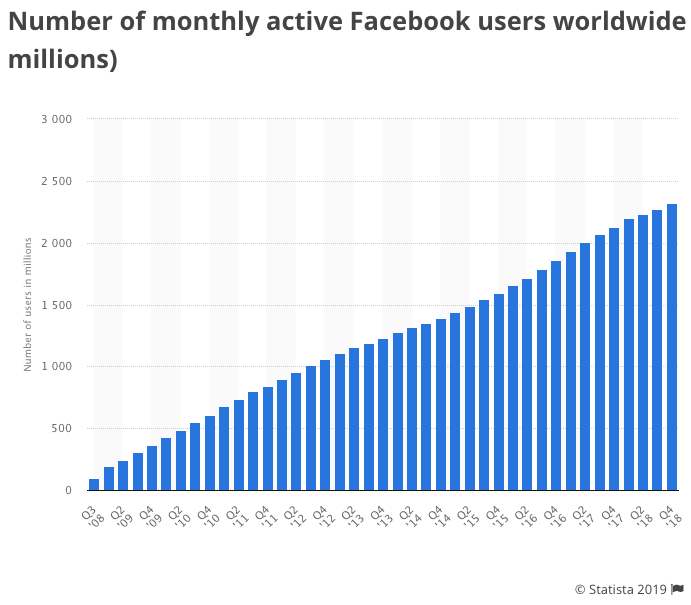
\includegraphics[width=\linewidth]{img/facebook-growth.png}
  \caption{Facebook Growth}
  \label{fig:FacebookG}
\end{figure}

In early 2000 is the year social media sites we know today started out and came into their own. Sites such as Facebook(2004), Reddit(2005) and Twitter(2006) all launched in the early 00's and are still very active today. These sites quickly gained an audience from people who wanted a more involved experience. These sites offered profile pages the user could customize and have users interact with one another. Facebook for example is the most popular social media site today (2019) expanding year over year in terms of users. 

Facebook has remained relevant through expanding their market and language options to make it more inclusive for people outside the western hemisphere where it first took off. which allowed it to incrementally increase its user-base year over year.

Sites early on like MySpace(2003), Flickr(2004) and Bebo(2005) all gained traction but rapidly fell out of use once more competition came into the market such as Facebook and Twitter.

\section{Modern Social Media}
Modern social media is constantly changing and is a market of "innovate or die". Social media sites are always trying to innovate in order to keep the audiences they've built over the years. An example is when Snapchat came into the market Facebook tries to create its own version of Snapchat stories in order to keep users on their platform.

Modern social media sites have their own perks that keep people using a different variety of social media sites and applications. Facebook is more of a personal social media between people you know or have met. Twitter is used to keep in up with people you would like to know about such as celebrities. Reddit is a post aggregator that is more of a classic forum from the early days of the internet. Instagram is a picture sharing application where you can follow friends and celebrities alike. All these social media site are different enough and offer a unique approach that they have been able to survive together. 

\section{Staying Relevant in our Ever-changing World} 


\begin{itemize}
\item Provide a context for your project.
\item Set out the objectives of the project
\item Briefly list each chapter / section and provide a 1-2 line description of what each section contains.
\item List the resource URL (GitHub address) for the project and provide a brief list of the main elements at the URL.
\end{itemize}

\chapter{Methodology}
In this chapter we will explore the approaches followed to plan, organise, manage and develop the project. We will discuss the methodologies that were adapted and combined to complete the research and development of the project along with why they were implemented. This section aims to give insight to the reader how the project transformed from research to final software while collaborating as a team.

Throughout our four years at GMIT a major emphasis was always placed on the importance of software development methodologies and the importance of choosing the most suitable methodology for a given project;. There are numerous  methodologies that have all been extensivly explore such as Waterfall, RAD (Rapid Application Development) and Extreme Programming to name a few. For this project we chose the main modern leader also based on the methodologies used by our employers, a concept known as Agile programming.


% ========================== Development approach  ========================== 
\section{Agile development approach}
Agile Software Development is a concept that allows a product be delivered to the customer in incremental releases while also being highly flexiable, allowing requiremnts to change and the scope of the project to increase without major consequences on the design or current task.

\begin{figure}[!htb]
  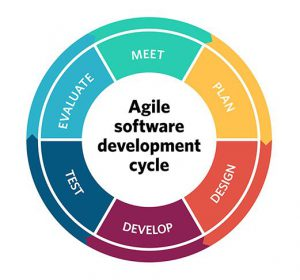
\includegraphics[width=\linewidth]{img/agile.jpg}
  \caption{Agile Methodogly}
  \label{fig:AGILE}
\end{figure}

We chose Agile as it stood out and had many benefits to our own project:

\begin{itemize}
\item Continuous Integration
\item Frequent feedback from customer 
\item Evolving requirements
\item Node.js
\end{itemize}

Firstly as we were exploring all new languages, frameworks and libraries Agile allowed us to easily continuously integrate new features as our knowledge portfolio grew. Another major advantage was that this approach allowed us to have a working model every week rather than releasing the project in one release as would be in the Waterfall methodology. This alone gave us the opportunity to review each weeks progress while also receive continuous feedback from our mentors.

From the outset of the planning phase the main requirements and features of the software were identified. Subsequently we broke these features down into sub tasks which enabled complex tasks to be completed with simplicity.   


% ========================== KanBan  ========================== 
\subsection{KanBan}
The Kanban Method is a means to design, manage, and improve flow systems for knowledge work. The method also allows organizations to start with their existing workflow and drive evolutionary change. They can do this by visualizing their flow of work, limit work in progress (WIP) and stop starting and start finishing.

The Kanban Method gets its name from the use of kanban - visual signaling mechanisms to control work in progress for intangible work products.

% ========================== Version Control  ========================== 
\section{Version Control}
Use of github, branches , KanBan project section to track progress

% ========================== Choice of tech  ========================== 
\section{Choice of tech }
tech used and why
 Selection criteria for algorithms, languages, platforms and technolo-gies.
 
% ========================== Testing , pass fail metrics  ========================== 
\section{Testing , pass fail metrics}
how we planned to test, what did we deternmine wwas a pass or fail

Check out the nice graphs in Figure \ref{tikz:graphs}, and the nice diagram in Figure \ref{tikz:mydiagram}.

\begin{figure}
  \centering
  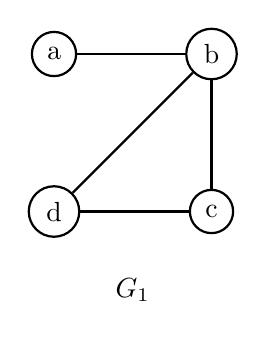
\begin{tikzpicture}
  \begin{scope}[every node/.style={circle,thick,draw}]
  \node (a) at (0,2) {a};
  \node (b) at (2,2) {b};
  \node (c) at (2,0) {c};
  \node (d) at (0,0) {d};
  \end{scope}
  \begin{scope}[every edge/.style={draw=black,thick}]
  \path (a) edge (b);
  \path (b) edge (c);
  \path (b) edge (d);
  \path (c) edge (d);
  \end{scope}
  \node () at (1,-1) {$G_1$};
  \end{tikzpicture}
  \hspace{1.5cm}
  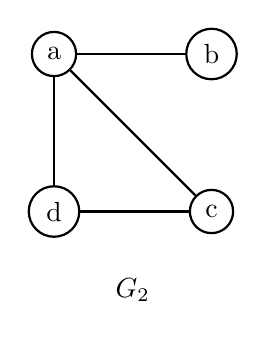
\begin{tikzpicture}
  \begin{scope}[every node/.style={circle,thick,draw}]
  \node (1) at (0,2) {a};
  \node (2) at (2,2) {b};
  \node (3) at (2,0) {c};
  \node (4) at (0,0) {d};
  \end{scope}
  \begin{scope}[every edge/.style={draw=black,thick}]
  \path (1) edge (2);
  \path (1) edge (3);
  \path (1) edge (4);
  \path (3) edge (4);
  \end{scope}
  \node () at (1,-1) {$G_2$};
  \end{tikzpicture}
  \caption{Nice pictures}
  \label{tikz:graphs}
\end{figure}


\begin{figure}
  \centering
  \begin{tikzpicture}[node distance=6cm]
  \node (a) [rect] {A Big Blue Block};
  \node (b) [oval, right of=a] {And His Oval Friend};
  \draw [line] (a) -- (b);
  \end{tikzpicture}
  \caption{Nice pictures}
  \label{tikz:graphs}
\end{figure}
\chapter{Technology Review} \label{techreview}
This chapter will cover the technical side of our project, by looking back on the technologies that made up the final revision of the project. We will explain the different technologies we added and how they were implemented through the project. We will look over the web stack we used and the technologies we added in order to create a more robust and useful social media site. We will go over why we used the given technologies and the benefits we saw in them over others.

% ========================== Framework  ========================== 
\section{MEAN STACK/Framework} \label{meanstack}
The mean stack is intended to provide a simple and fun starting point for cloud native full-stack JavaScript applications. MEAN is a set of Open Source components that together, provide an end-to-end framework for building dynamic web applications; starting from the top (code running in the browser) to the bottom (database). 

The stack is made up of:

\begin{itemize}
\item MongoDB
\item ExpressJS
\item Angular
\item Node.js
\end{itemize}

Early in development when we were brainstorming, we decided to do a full stack development. The next step after this decision was to figure out how to carry out this task. We looked into full development stacks such as the MERN stack (MongoDB, ExpressJS, React, Node.js), MEAN stack (MongoDB, ExpressJS, Angular, Node.js) or doing a Java-based development stack (Spring boot, Angular, MongoDB). After lots of discussion and input from supervisors, we decided to not go with the Java-based development stack. We then took a deep dive into the difference between the MEAN/MERN stack to decide what route we wanted to take and start development as soon as possible. After looking into React JSX vs Angular HTML templating and experimenting with the two stacks we finally decided that the MEAN stack was more inline in what we wanted to learn.

Once we knew what stack we were using and how to use it in a basic form from our prototyping stage, we moved onto breaking the stack down to each component and getting to know each component better, so when full development starts we would have a better understand how the entire stack operates and interacts with each component. This gave us a greater understanding of how each component operated and allowed us to plan out how each component would operate from top to bottom. 

\subsection{MongoDB}
You may know what MySQL and other relational databases are. MySQL is analogous to a spreadsheet, it has name columns and rows of rows of data. Every database "tool" shows the data as a spreadsheet (Microsoft Access). Data can be linked through special functions such as a "JOIN" mechanism to allow the user to built meta spreadsheets. 

MongoDB is a database and not a database tool (Mongo Compass), instead of a spreadsheet like MySQL it is more like a folder of documents. The contents of the "folders" are not checked to see if the new file differs from the current file format. This sounds like an inefficient system but all these folders are called collections in MongoDB. The collections are usually grouped by how the user would group MySQL tables. While MongoDB can contain keys like MySQL there is no built-in functionality in order to join documents together in order to retrieve related data in another collection.

Databases are classified into two categories of SQL and NoSQL. MySQL is an example of an SQL database, and MongoDB is an example of a NoSQL database. MongoDB is very reliable as its very hands off and gives the user the responsibility for how data is saved and read. If a user adds another entry into the collection that doesn't match the other entries MongoDB doesn't inform the user that the data is not in the correct format as collections do not have definitions and leave that responsibility to the user. The same goes for joining two collections together. The joining is left up to the user on how they carry that out, usually, the user would create an ID which is present in both collections in order to 'join' them together.

MongoDB is so hands off about how users read and write to the database it stops the frequently used attack on SQL databases called SQL injection. SQL injection occurs when the user directly interacts with the database which allows them to manipulate their input to test the database. MongoDB doesn't have this problem as its hands off the reading data to the user to the point where a search for that data will include the statement but nor process the statement as such.

MongoDB uses the JSON standard to store data. The JSON data is then classified into a collection as we discussed above. 

Example of how a JSON entry in a collection could look like:

\begin{minted}{js}
{
    "username": "Smithy",
    "password": "smith123",
    "name": {
        "first_name" : "John",
        "second_name" : "Smith",
    }
}
\end{minted}

\subsection{ExpressJS}
ExpressJS is a minimalistic web framework built for Node.js that waits for the browser to connect so the server can send process the request and send back the relevant form (JSON, HTML, Raw Text, ETC...). Without ExpressJS the user must handle creating a server, handling routing all manually.

ExpressJS relies on APIs made available by Node.js. ExpressJS cannot exist without Node.js. ExpressJS is a thin layer over Node.js which makes developing servers and routes much easier. ExpressJS's main feature that makes it enticing to developers is how it serves dynamic content (Content that changes based on user requests). 

ExpressJS also has the capability to server components from frameworks such as Angular, Ember and React and process requests made by those components to update their content. ExpressJS makes Node.js development easier, especially when creating APIs that front-end apps use. Express makes it easier to unify the front-end apps and the API.

ExpressJS was an easy pick for the project as it easily integrates Node.js and rapidly decreased the time it would take to get the server side API up and running.

\subsection{Angular}
Angular is a front-end web framework built on top of JavaScript, it is used to develop single-page web applications. Single-page web frameworks (Angular, React, Ember) are websites which have all the functionality of a multiple page website without having the need to refresh the browser when moving from page to page. Single-page web development frameworks have become increasingly popular in the last few years due to how reactive they are. Pages react very fast and fluidly making user interaction with the website more positive than refreshing when moving to another page on the same website. 

Angular has been around since 2010 with the release of AngularJS. Later version came out and greatly improved upon the idea with Angular 2+ or Angular v2. This version would be improved upon and maintained by Google with the latest release being Angular 7 in late 2018. Despite angular being around for nearly 10 years, it has only been in the last few years where it has come into its own and seen real competition from other single-page frameworks such as React and Ember.

We chose Angular because of its integration with Node.js/ExpressJS which allowed us to get prototypes for testing the MEAN stack up and running very quickly and let us play around with the different functions it offered as part of its component-based setup. Within a week we had the entire MEAN stack in a functional state where Angular was served with Node.js/ExpressJS and then send and received data from the API served by the Node.js/ExpressJS server.

\subsection{Node.js}
Node.js is a cross-platform JavaScript run-time environment that allows developers to run JavaScript outside the browser. This framework is a huge deal for JavaScript. Node.js allows developers to perform actions with JavaScript on the developer's local machine like they would with other programming languages. What makes Node.js so beloved by developers is the built-in functionality of Node.js. Node.js has built-in HTTP function to allow Node.js to run HTTP actions all within the environment. This built-in HTTP functionality has made Node.js extremely popular and given the rise to isomorphic web applications and due to the fact that Node.js can run as a server back-end using JavaScript and have JavaScript on the front-end meaning there is the opportunity for the two to share code between them reducing testing and maintenance.

Node.js is a great framework due when paired with a front-end framework such as Angular, and a database such as MongoDB. When using a setup like this the entire web stack is a JavaScript based and allows the user to easily manipulate data from top to bottom.

The reason we picked Node.js is because of its ease of use and how rapidly we could get a working HTTP server up and running. Node.js also made a lot of sense when paired with Angular which was the front-end framework we picked. Node.js makes developing HTTP servers easy, which allowed us to spend more time on setting up other features such as user authentication and the Reddit API. 

Here is an example of all the code needed to create a simple Node.js server. This code will display "Hello World!" to the user in the browser on port "8080".
\begin{minted}{js}
var http = require('http');

//create a server object:
http.createServer(function (req, res) {
  res.write('Hello World!');
  res.end();
}).listen(8080);
\end{minted}

\subsubsection{Node Modules}
Node.js allows developers to develop and use packages which provide the developer with more functionality.

\begin{figure}[H]
  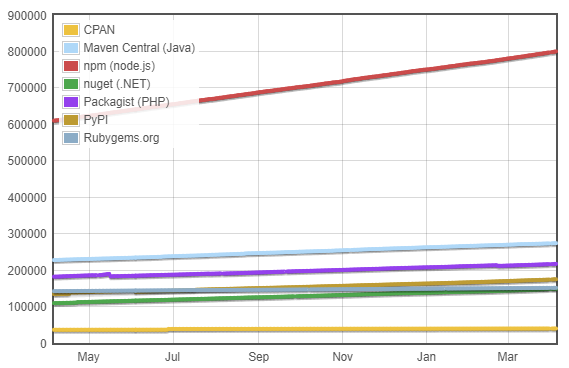
\includegraphics[width=\linewidth]{img/moduleCount.PNG}
  \caption{NPM Package Count}
  \label{fig:NPM}
\end{figure}

NPM is the world’s largest software registry. NPM allows developers access to lots of packages for all sorts of development such as packages for Node.js, Angular, MongoDB and even developing Alexa skills. NPM allows developers to upload custom packages that they have developed and give access to other developers to use it in their system.

Node modules is a powerful resource with lots of packages that adds great functionality to the developer's project such as user authentication with Passport.js.

% ========================== DEPLOYMENT  ========================== 
\section{Deployment}
For code deployments we looked at numerous cloud service provides to figure out what would be the best service to take use of for our project. We looked at Google Cloud, Heroku and AWS as the cloud service providers. Although these are only a fraction of the cloud service providers online, we found they were received very well by our supervisors as a way of deployment. 

We ruled out Google cloud after lots of debate on how to move forward with deployment. The reason to remove Google Cloud first was we felt that we wanted to get a greater understanding of a different cloud service provider as we already had experience with Google Cloud. After ruling our Google Cloud we were left with Heroku and AWS. After researching more into both options and figuring out what would better with our project we decided to go with AWS because of AWS's Elastic Beanstalk. AWS Elastic Beanstalk is a system provided by AWS for deploying and scaling web applications and services developed with Java, .NET, PHP, Node.js, Python, Ruby, Go, and Docker on familiar servers.  Because of AWS's Elastic Beanstalk and us using the MEAN stack, it was an easy way to deploy our project, and an easier way to expand the project if we wanted to go commercial with the website.

% ========================== STANDARDS  ========================== 
\section{Standards}
\subsection{JSON}
JavaScript Object-Notation is a specification for Serialization a data object. Serialization is a is the process that turns a price of code into a string of characters in order to transmit it. 

The basic idea is that if you want to transmit a piece of data that has attributes such as name, address, age, etc and turning it into a string.

An example of converting an object to JSON specification would be for example this object of the user.

\begin{minted}{java}
class user{
    string username;
    string password;
    int age;
}
\end{minted}

Let's say the user created an instance of this object and set the values to "Smithy", "smith123" and "25". To send this instance over to another machine in a standard the other machine we can't just send it in raw text using HTTP so we need to serialize the data before transfer using the JSON specification. 

The JSON string would look like this when the class is serialized:
\begin{minted}{js}
{
    "username": "Smithy",
    "password": "smith123",
    "age": 25
}
\end{minted}

Once the class is correctly serialized, the object can be added to the HTTP request to be sent over to the other machine. The JSON object would be added to the body of the HTTP request for the machine on the other end to retrieve and do with as it needs.

An example of it in the body would be:
\begin{minted}{js}
{ "user": {"username": "Smithy","password": "smith123","age": 25} }
\end{minted}

With this machine-readable string, I can now retrieve the data by deserializing the string back into an object. This all works because of the JSON specification which creates a standard for how to serialize and deserialize the JSON object.

\subsection{REST}
Representational State Transfer or REST is a guideline for sending information on the Internet. It is an architectural system that has gained in popularity over the years. RESTful web services are a common way of accessing an online API. Users can make multiple different requests through one URL with certain parameters. The REST architecture design has an emphasis on nouns to tell what the resource the user is trying to access is and how the resource is going to be affected by HTTP modules. 

Let's say a developer is making a system that accesses a database that requires read, write, update and delete functions. A REST URL could be for example "/api/account". Using this URL we can create a RESTful resource that the developer has access to with all these functions.

Using the REST specification we can create these four functions in the one URL route or resource by using the different HTTP methods (GET, POST, PUT, DELETE) for each function. All four HTTP requests to do with a user account would use the "/api/account" route to read, write, update and delete the user's data.

The REST specification streamlines the development of a server API and makes managing the API on the server as well as the application using the API much easier.

% ========================== REST API  ========================== 
\section{REST API}
The REST API we setup is intended to give access to all aspects of the project in a public format. The REST API is used by Angular which gives the user a visual representation of the data being sent and received by the REST API. Some routes are protected by Passport.js which encodes user data used to access certain routes such as update profile picture or password.

A big benefit of the API is all functionality of the application is available from the REST API. This allows for us to if we decided to, add a mobile application or create a monitoring tool to see the data and analyze it.

\subsection{Security}
Routes altering data (POST, PUT, DELETE) requires the user to be authenticated to prevent data being altered by another user. We authenticated certain routes such as create a post to check who is creating this post, and to link to their profile but also so only they can post in their name. Authenticating routes such as comment, post, settings and following was a big part of the planning stage as we needed to figure out a way to stop intrusive behaviour from outside sources abusing the API.

To add a layer of security to user requests and ensure no malicious requests are made by other user trying to impersonate another user we added a Node.js import called PassportJS. PassportJS is authentication middle-ware for Node.js. PassportJS allows

\subsection{Swagger}
Swagger is an open source software framework sponsored by SmartBear. Swagger is used to create, document and consume  RESTful Web services. Swagger offers an easy way to document RESTful Web services by using Swagger documentation definitions and Swagger UI to document an API and give example on how the API works. Swagger works by having the developer add comments similar to java-docs in order to document a route telling swagger the components of the route and the model it uses. Giving swagger this information swagger will use the data to create a JSON object with all the data about the API in a format that can be used by the developer for other means or to be used in conjunction with swagger UI, which we will discuss later.

\subsubsection{Swagger.json}
As we discussed above Swagger is used to document a route. But how does it do that? Swagger creates a JSON object which it hosts at a given route in order to be accessible by developers for their own purposes, or by using Swagger UI.

The JSON part of Swagger is where the swagger documentation is rendered into a machine readable format.

\begin{minted}{js}
{
    info: { 
        title: "Node Swagger API",
        version: "1.0.0",
        description: "Api file for swagger"
    },
    host: "34.243.30.50:3000",
    basePath: "/",
    swagger: "2.0",
    paths: {},
    definitions: {},
    responses: { },
    parameters: { },
    securityDefinitions: { }
}
\end{minted}

Above is an example from the hosted project on AWS. As we can see this is a very basic model for without any route or definitions. Swagger includes basic information about the API such as the host and general Swagger information such as version and title. Swagger includes the host and base-path used by the API, with a list of definitions and paths about each API route.

\begin{minted}{js}
paths: {
    /api: {
        get: {
        tags: [
            "books"
            ],
            description: "Returns all books",
            produces: [
            "application/json"
            ],
            responses: {
                200: {
                    description: "An array of books",
                    schema: {
                        \$ref: "#/definitions/book"
                    }
                }
            }
        },
    },
},
\end{minted}

An example of one of the paths contained in the paths object array. In paths we have a list of paths documented using Swagger, these paths contain information about the path such as the title in which the path could be classified under, example above is 'Books'. With the title we can classify different paths that may handle something to do with 'books' and thus we may want to organizes the paths under 'books'. The path also contains the schema used which is very important in order to understand how the API route operates. Does the path return JSON?, XML?, raw text?

\begin{minted}{js}
definitions: {
    book: {
        properties: {
            isbn: {
                type: "string"
            },
            title: {
                type: "string"
            },
            author: {
                type: "string"
            },
            description: {
                type: "string"
            },
            published_year: {
                type: "string"
            },
            publisher: {
                type: "string"
            }
        }
    }
},
\end{minted}

Using the definition in conjunction with the path we can get a better picture of how to API route works and what data is needed for it to operate correctly. The definitions contains definitions for each route and each definition inside definitions contains properties which describe the routes data and what type of data each property is.

\subsubsection{Swagger UI}
Swagger UI is a visual representation of the API documented using Swagger. Swagger UI is a great as it enables developers to save a lot of time in documenting an API, as it uses the Swagger JSON to visualize the API. 

\begin{figure}[H]
  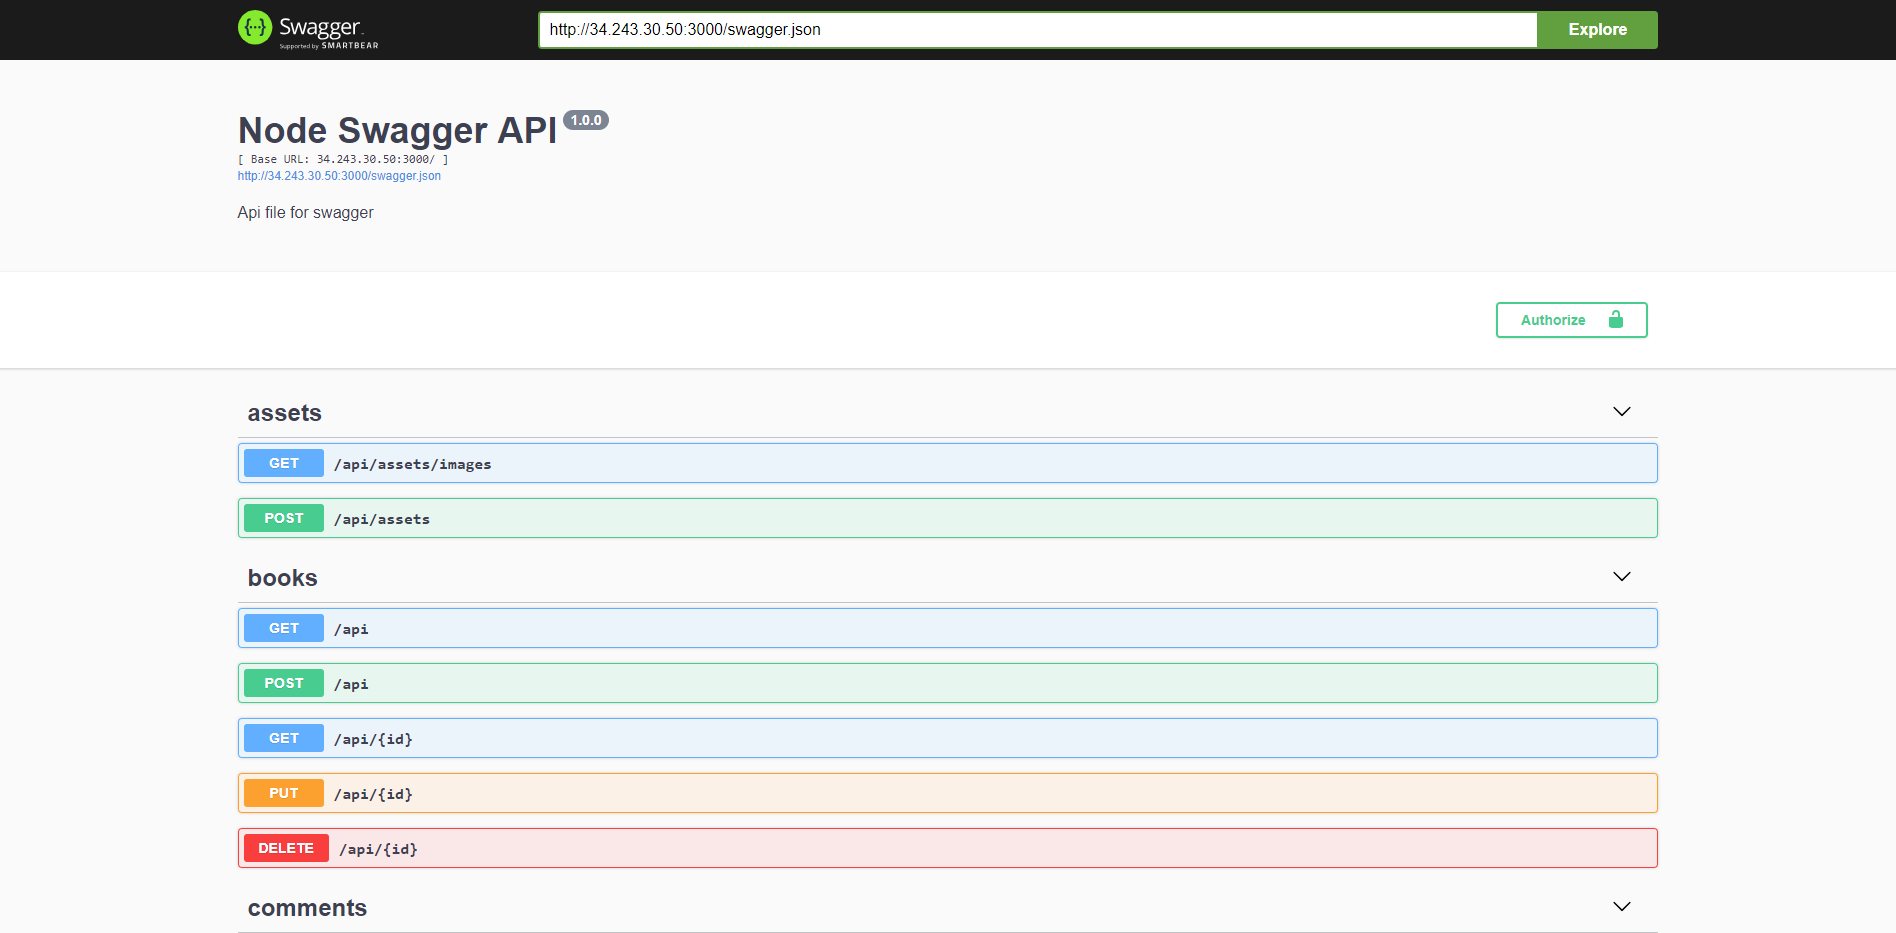
\includegraphics[width=\linewidth]{img/swaggerUI.PNG}
  \caption{Swagger UI}
  \label{fig:NPM}
\end{figure}

Using Swagger UI we can use the hosted JSON from the Swagger Documentation to display the available routes in the API. Each route is categorized and sorted using the Swagger JSON. Each option under the category will use the path and definition of the Swagger JSON to create a visualized representation of the API and allow testing of the API.

% ========================== Languages ========================== 
\section{Languages}
\subsection{JavaScript}
JavaScript is the backbone of the web. JavaScript is responsible for front-end web development processes. Without JavaScript a web page would have no functionality to communicate with the server-side functions in order to save or read dynamic data. JavaScript runs the web, both front-end with JavaScript or TypeScript. 

A very basic way to think of JavaScript is that HTML is your bone structure. It holds everything together with a solid foundation. CSS is your skin, it's what everyone sees and interacts with. So JavaScript is your brain, heart and other organs that make you, you. JavaScript is what makes everything function in an effective way.

\subsubsection{Database}
JavaScript is found in the database with MongoDB, which stores data using JSON (JavaScript Object Notation). MongoDB saves database entries using JSON to store elements of that collection. As we explained earlier what JSON is and how it stores classes into objects.

\subsubsection{Server-Side}
On the server-side we used Node.js. Node.js as we discussed above is what allows JavaScript to run outside the browser. JavaScript was used as the serer-side processing which handled routing for the API and for the Angular front-end.

\subsubsection{Front-End}
The front end section of the web application uses TypeScript which is a super-set of JavaScript which we will talk about in greater detail below.

in the server-side API handling routing for the web application. 

\subsection{TypeScript}
TypeScript which is a super-set of JavaScript. JavaScript code is valid in a TypeScript environment, with some exceptions. A huge benefit over JavaScript is that TypeScript made it harder to create bugs and made JavaScript more manageable in larger systems.

\vspace{5mm}

JavaScript:
\begin{minted}{js}
let name = 'TechBook',
users = 500,
isThreeTier = true;
\end{minted}

TypeScript:
\begin{minted}{js}
let name: string = 'TechBook',
users: number = 500,
isThreeTier: boolean = true;
\end{minted}

The biggest change and most liked feature of TypeScript is variables are declared by using a variable type such as 'string', 'number' and 'boolean'. This is a big change over JavaScript where the variable type is interpreted as to how the developer manages the variable.

\subsection{HTML}
HTML (Hypertext Markup Language) is a markup language for creating web pages. HTML uses tags to define what sections of the web page do what. 

HTML Example:
\begin{minted}{html}
<h1> Title </h1>
<p> Paragraph</p>
<a href= "github.com"> Link </a>
\end{minted}

HTML Rendered: \\
\textbf{Title} \\
Paragraph \\
\href{http://www.sharelatex.com}{Link}

\vspace{5mm}

Every web-page on the internet is a hypertext document. A hypertext document differs from a raw text document by allowing images, formatting and links. HTML is is what hold all the components of a web-page together. 

\subsection{LaTeX}
LaTeX is a text processor that is built around a markup language. Like HTML LaTeX uses tags to define a command or action to display text in a certain way. These tags work very similar to HTML where these tags are only seen on the source of the document and are hidden when the document is compiled into a format such as a PDF.

LaTeX Example:
\begin{minted}{tex}
\chapter{Technology Review}
\section{Languages}
\subsection{LaTeX}
Some text about LaTeX
\end{minted}

LaTeX would then compile this text into a document, like this one, where it renders the chapter the section and subsection of that chapter and would compile the table of contents to include the new chapter and sections.

% ========================== Styling and UI  ========================== 
\section{Styling and UI}
In this section we will talk about the different technologies we used to develop the front-end user interface for our website. 

User interfaces are an extremely important aspect of website design. As more people have access to the internet using different hardware and software to access website, it has become harder to develop a streamlined user interface that works across all devices. 

Things that can affect user interface development:
\begin{itemize}
    \item Aspect Ratio
    \item Resolution
    \item Browser
    \item Mobile/Desktop
\end{itemize}

Creating an intuitive user interface that works across most devices is difficult because of the above reasons. Using different technologies we will discuss below often these technologies take care of many of these issues. As long as the developer keeps them in mind and tries to use the functionality they provide to make the website accessible to as much people as possible.

Mobile has become a major part of accessing the internet as smart-phones have become a bigger part in peoples lives and can be used anywhere. Developing a user interface that works on both desktop PCs and mobile smart phones can be challenging. Developing a website that works on both devices was very important to us to keep up with modern trends.

\subsection{CSS}
As we discussed briefly in the previous section, CSS is the  skin of the project. It's what most sites use to make their appearance more professional and not just a wall of text and buttons. CSS stands for 'Cascading Style Sheets. It's used by nearly all websites to improve their appearance and makes a website stand out from each other.

\begin{figure}[H]
    \centering
    \begin{minipage}{.50\textwidth}
      \centering
      
\includegraphics[width=.9\linewidth]{img/facebookCSS.PNG}
      \captionof{figure}{CSS Facebook}
      \label{fig:aboutPC}
    \end{minipage}%
    \begin{minipage}{.50\textwidth}
      \centering
      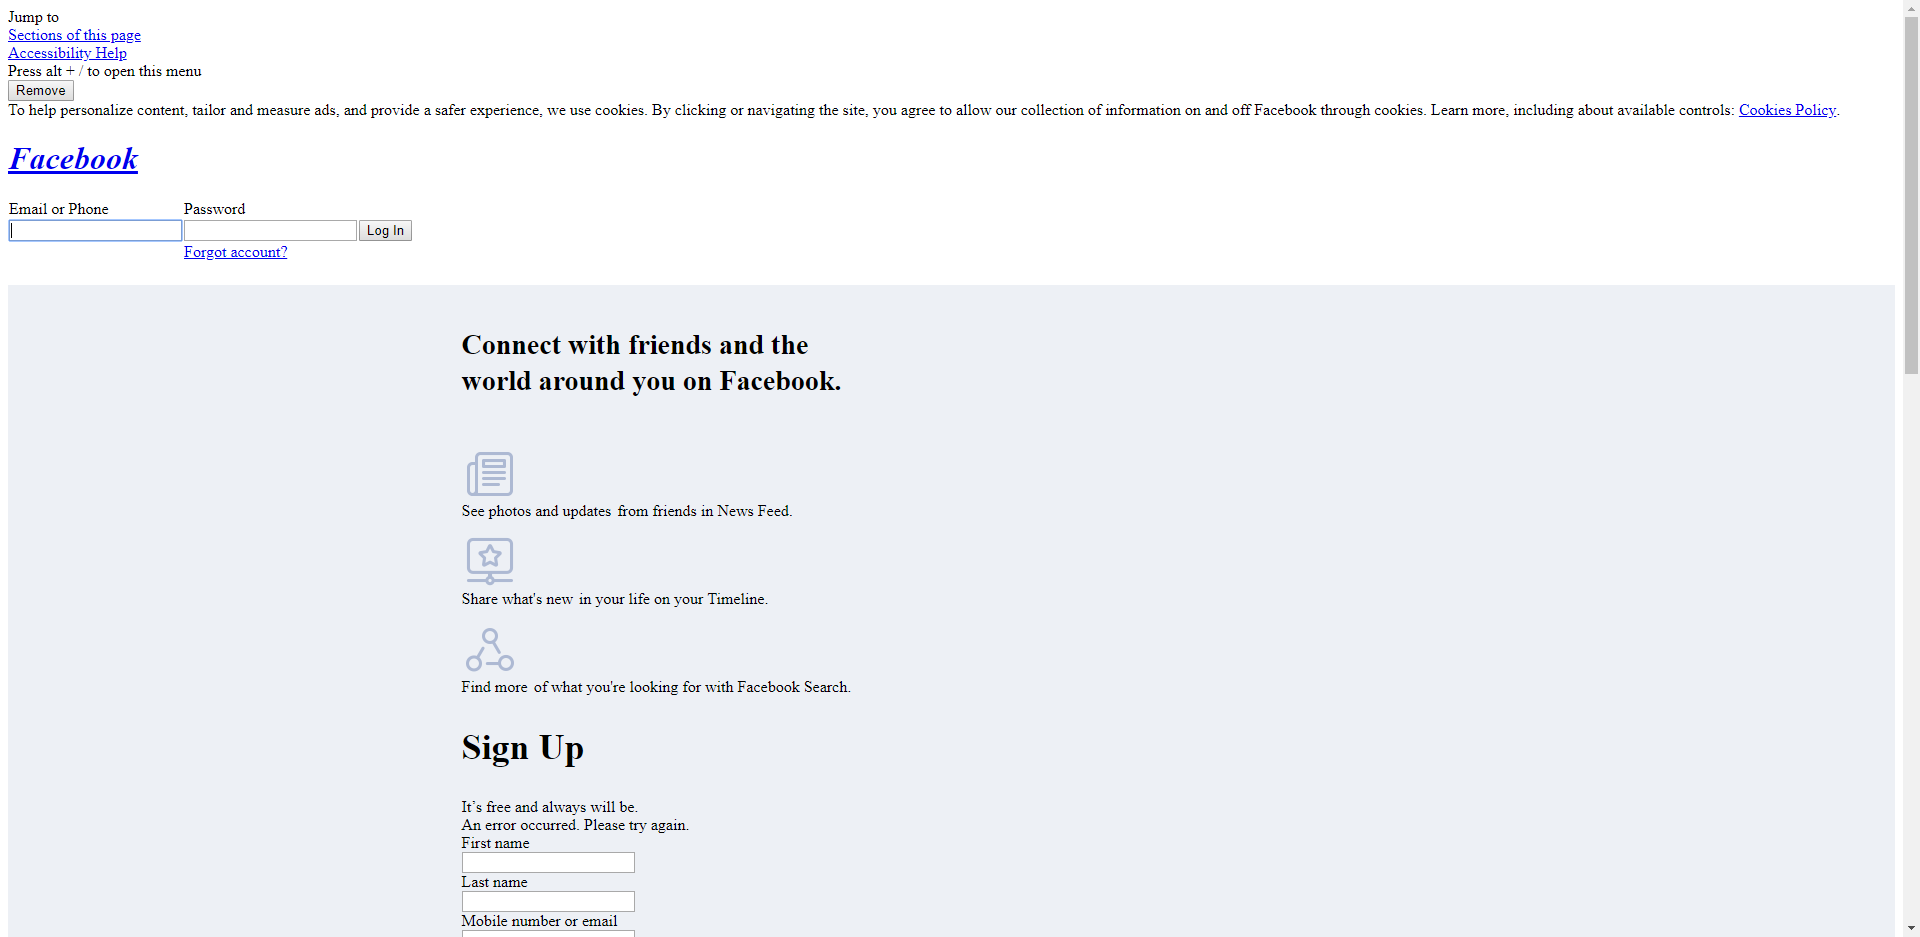
\includegraphics[width=.9\linewidth]{img/facebookNoCSS.PNG}
      \captionof{figure}{No CSS Facebook}
      \label{fig:aboutMobile}
    \end{minipage}
\end{figure}

As we can see above is an example of what the web would look like without CSS. Facebook would go from a modern looking website to a very basic text website with a few images spread around.

CSS is an extremely easy tool to grasp, but takes time to master, especially with the different screen sizes, aspect ratios and resolutions.

\subsection{Bootstrap}
Bootstrap is a pre-written library of CSS files that enables developers to rapidly develop the UI for their website. Bootstrap also allows developers to make their own CSS files and build on top of Bootstrap to refine a website design.

Bootstrap is great for quickly developing prototypes for website as it takes a lot of the grunt work and allows the developer to concentrate on getting the functionality right. CSS offers a great way to style a website, but often it can be hard to get a certain function to work correctly. Bootstrap takes care of a lot of the functionality the developer may need such as a sticky navigation-bar. Instead of the developer making a their own sticky navigation-bar using CSS and JavaScript, they can off-load that work to Bootstrap which will do all that using the specified Bootstrap class.

\subsection{Angular Material}
Angular Material is developed bu Google and was developed to meet the demand of their new design spec 'Google Now'. Google Now laid out a grid-based website with animations and responsive cards, which was used used until the serviced was discontinued.

\begin{displayquote}
"Unlike real paper, our digital material can expand and reform intelligently. Material has physical surfaces and edges. Seams and shadows provide meaning about what you can touch" - Matias Duarte, VP of Design at Google
\end{displayquote}

Angular Material was birthed from the now defunct service. Angular Material was made to create a Bootstrap like alternative. Although Angular Material is an alternative to Bootstrap to develop front-end user interfaces, Bootstrap is often used in conjunction with Angular Material.

% ========================== Other Technology's  ========================== 
\section{Other Technologies/Development environment}
In this section we will go over the technologies we used to develop and test the web application.

\subsection{Visual Studio Code}
\begin{figure}[H]
  
\includegraphics[width=\linewidth]{img/opengraph-home.png}
  \caption{Visual Studio Code View}
  \label{fig:VSC}
\end{figure}

Use used Microsoft's Visual Studio Code as an integrated development environment as it was perfect for what we needed. We needed an integrated development environment that didn't just support one language. We needed one that supported, JavaScript, TypeScript, HTML, CSS and LaTeX. Visual Studio Code offers a specialized extensions that make developing with these technologies more initiative.

\subsubsection{Extensions}
Extensions for Visual Studio Code are add-ons developed by others to make the development environment in Visual Studio Code better for a specific task.

\paragraph{HTML CSS Support}
HTML CSS Support extension is just what it sounds like, it adds better support for HTML and CSS in Visual Studio Code. Although you can easily write code in Visual Studio Code for HTML and CSS this extension adds features that make the development of HTML and CSS like developing Java using Eclipse would.

\begin{itemize}
    \item Class attribute completion
    \item Id attribute completion.
    \item Supports Zen Coding completion for class and id attributes.
    \item Scans workspace folder for CSS and SCSS files.
    \item Supports remote CSS files.
\end{itemize}

It's small features like these that make developing HTML and CSS a little easier, especially when developing a full stack website. HTML CSS Support extension made developing with HTML and CSS feel more natural in Visual Studio Code.

\paragraph{JavaScript (ES6) Code Snippets}
JavaScript (ES6) Code Snippets is an extension which adds shortcuts for common JavaScript and Typescript functionality such as for loop, console log and class constructors.

Supports:
\begin{itemize}
    \item JavaScript (.js)
    \item TypeScript (.ts)
    \item JavaScript React (.jsx)
    \item TypeScript React (.tsx)
    \item Html (.html)
    \item Vue (.vue)
\end{itemize}

The extension supporting both JavaScript and TypeScript was what sold us on the extension as those two languages made up the majority of our code-base. 

Using the extension is very easy once you know a few of the shortcuts and how to use them. An example of use would be typing 'clg' and pressing TAB which would convert 'clg' to 'console.log();'. The extension made getting something setup easy such as 'fof' and pressing TAB becoming 'for(const item of object) {}'. Although very basic, it made writing small code snippets easier and more in line with IDEs such as Eclipse with 'sysout' and then pressing CTRL-SPACE which produced 'System.out.println'.

\paragraph{LaTeX Workshop}
LaTeX Workshop was used early on in development. The extension provided live PDF view to see how changes looked and has came with quality of life features such as shortcuts.

LaTeX Workshop made developing LaTeX in Visual Studio Code easier with the features it provided.

\subsection{Browsers}
We used two primary and popular browsers during development. We didn't want to just use one as a feature might work for one but not the other. This wasn't a big problem as Angular handled much of the primary features with each browser, the bigger problem with trying to get cross browser support was CSS settings and how each browser would interpret them. We used chrome, Internet Explorer/Edge and Firefox as they had the largest market-share.
\chapter{System Design}
In this chapter we will discuss the architecture and design of the \textbf{TechBook} system. In the following sections we will present code snippets and visual diagrams to help portray a basic understanding of the application design. The architecture is modeled on what is known as the MEAN stack and which resembles a three tier architecture. MEAN is a free open-source software stack for building dynamic websites and supports the MVC (Model View Controller) architecture. The contents of this chapter will be seperated into the Data Tier, Logic Tier and Presentation Tier.




\begin{figure}[H]
\begin{minipage}{.5\textwidth}  %listing bloc will have 50% of the line width 
\lstset{linewidth = 4cm, breaklines=true} %set your listing lines widths, and set breaklines to true
\begin{itemize}
\item Database \textbf{MongoDB}
\item Server \textbf{Node.js/express}
\item Client \textbf{Angular.js}
\end{itemize}

\end{minipage}
\qquad %space between listing bloc and the figure
\begin{minipage}{0.4\textwidth} %figure will have the remaning 40% of the line width
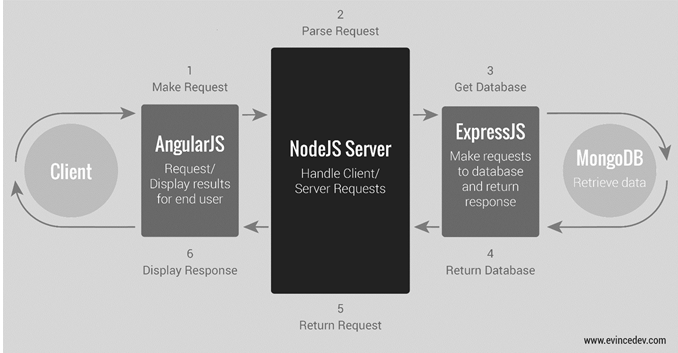
\includegraphics[scale=.4]{img/mvc.png} %the image must be resized or scaled if needed
\caption{MEAN Stack}
\end{minipage}
\end{figure}

% ========================== Databases ========================== 
\section{Database}
For the database adapting the MEAN architecture we used MongoDB.

\subsection{Mongoose}
Harnessing the true power of the Mean stack we used the mongoose object modelling package for Node. Mongoose enabled us to have access to the full suite of MongoDB commands to perform CRUD (Create, Read, Update, Delete) operations. 


To use mongoose we used the following command in the project directory to add it to our Node project:
\begin{lstlisting}[language=DOS]
npm install mongoose --save
\end{lstlisting}

Once the package was installed we have to access it in our project :
\begin{lstlisting}[language=JavaScript]
var mongoose = require('mongoose');
\end{lstlisting}

Finally to connect to our MongoDB:
\begin{lstlisting}[language=JavaScript]
// Connect to the mongodb using settings from the config file
mongoose.connect(config.database, { promiseLibrary: require('bluebird') })
  .then(() =>  console.log('\x1b[32m%s\x1b[0m', 'INFO: Connection to database succesfull'))
  .catch((err) => console.error(err));
\end{lstlisting}

\subsection{Mongoose Schema}
Prior to performing CRUD operations we had to define our  mongooses models. These represent documents which can be saved, read and retrieved from our database. The Mongoose Schema is how we define attributes to these documents. To enhance security and the SRP(Single Responsibility Principle) numerous different models were defined and using keys enabled the ability to map relationships to other models.

\begin{figure}[H]
  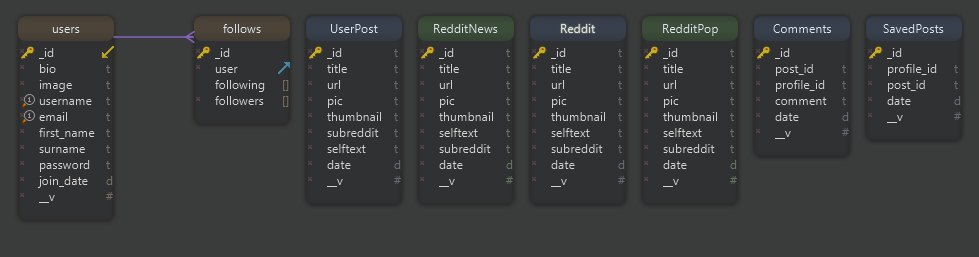
\includegraphics[width=\linewidth]{img/schemas.PNG}
  \caption{MongoDB models}
  \label{fig:schema}
\end{figure}

Figure ~\ref{fig:userscema} below shows how the UserSchema was defined in user.js. The schema was designed to add maximum functionality while also protecting the system from having invalid objects added to the database. There are a few things to note about this particular schema.
\begin{itemize}
\item \textbf{Uniqueness} : The \textit{username} and \textit{email} fields are set to unique. This ensures a user can only have one account per email and that the username will not not cause issues when a search query is performed.
\item \textbf{Required} : The \textit{username}, \textit{firstname},\textit{surname} and \textit{password} fields are required. These represent the bare minimum that must be initialised to have a valid account.
\item \textbf{Default} : The \textit{joindate},\textit{bio} and \textit{image} are set to default. This allows a faster user registration with a default image used, the join date set to the current date and a generic bio that can all be updated using the settings link.
\end{itemize}

\begin{lstlisting}[language=JavaScript,caption={Defining User Schema},captionpos=b,label={fig:userscema}]
// Schema used to 'filter' data to be stored in the 'UserSchema' collection in mongo
var UserSchema = new mongoose.Schema({
  username: {
    type: String,
    unique: true,
    required: true
  },
  email: {
    type: String,
    unique: true,
  },
  first_name: {
    type: String,
    required: true
  },
  surname: {
    type: String,
    required: true
  },
  join_date: {
    type: Date,
    default: Date.now
  },
  bio: {
    type: String,
    default: 'Tell me about yourself'
  },
  image:{
    type: String,
    default: 'profile.jpg'
  },
  password: {
    type: String,
    required: true
  }
});

\end{lstlisting}

\subsection{Password hashing}
To ensure the highest standard of security any confidential user information should never directly be stored in a database. Mongoose allows us to define functions using 'pre(function,functionToExecute)' that executes prior to saving a document. Bcrypt a node-module that simplifies hashing can be used to both encrypt and decrypt sensitive data. Combining the use of these technologies when a user account is created or modified, the password is hashed before saving the document and in turn the hashed value of the password is saved in the database thus protecting the origonal password being exposed in the event of a malicious attack.

\begin{lstlisting}[language=JavaScript,caption={Password Hashing},captionpos=b,label={fig:presave}]
// define pre hook for document
UserSchema.pre('save', function (next) {
  var user = this;
  // if password new or edited
  if (this.isModified('password') || this.isNew) {
    // generate a salt and process data for 10 rounds
    bcrypt.genSalt(10, function (err, salt) {
      if (err) {
        return next(err);
      }
      // generate a hash of password
      bcrypt.hash(user.password, salt, null, function (err, hash) {
        if (err) {
          return next(err);
        }
        user.password = hash;
        next();
      });
    });
  } else {
    return next();
  }
});

\end{lstlisting}
Ensuring the password is hashed is of major importance but equally as crucial is the ability to be able to compare the hashed value with a password entered by a user attempting to log in. To achieve this we were able to attach a comparePassword function to the UserSchema which executes the compare method from the bcrypt module and checks for a match between the password entered and the hashed password stored in the database as shown in Figure ~\ref{fig:passcheck}. 
\begin{lstlisting}[language=JavaScript,caption={Password Comparision},captionpos=b,label={fig:passcheck}]
// compare password for log in
UserSchema.methods.comparePassword = function (passw, cb) {
  bcrypt.compare(passw, this.password, function (err, isMatch) {
    if (err) {
      return cb(err);
    }
    cb(null, isMatch);
  });
};
\end{lstlisting}

\subsection{JSON Web tokens}
% ========================== Authentication ========================== 
\section{Authentication}
What database like

% ========================== API Calls ========================== 
\section{API/HTTP}
How we designed api calls/
insert info from swagger

% ========================== UI ========================== 
\section{Client UI}
The presentation tier is based on the Angular front-end web framework. In contrast to traditional multiple page web applications the Client is presented as a single page application in which components are injected into. In this section we will look at the Angular app structure, the services which allow us to interact with our node js server and the finished view of the pages.

\subsection{Angular folder structure}

\subsection{Angular Services}
The Angular services allow our application to interact and access data from our database via the node server. Thus keeping data retrieval separate to page functions. In the services we provide the logic to process HTTP requests to the API to perform CRUD operations on the data served by the Node.js/ExpressJS server. 

\subsection{Page views}
In this section we will look at some screen shots of the web application from the view of a PC web browser and on a Samsung Galaxy S6 mobile device. For each page a brief summary of the functionality of the page will be provided along with any input validation that was used. 
How we designed the ui
few screenshots off finished site

\subsubsection{Log in Page}
The log in page consists of of a username and password input box. In order to submit a login attempt both values must be supplied. The values are then authenticated on the server and if successful the server returns a JWT token that's stored in session storage and the user is redirected to the homepage view.  If the username is invalid the server will return a "Log in failed. User not found." error message to the view or in the case of an invalid password a "Incorrect password" message is returned.
\begin{figure}[H]
\centering
\begin{minipage}{.75\textwidth}
  \centering
  
\includegraphics[width=.9\linewidth]{img/ui/login_PC.PNG}
  \captionof{figure}{Web View}
  \label{fig:loginPC}
\end{minipage}%
\begin{minipage}{.25\textwidth}
  \centering
  
\includegraphics[width=.9\linewidth]{img/ui/login_MOBILE.PNG}
  \captionof{figure}{Mobile view}
  \label{fig:loginMOBILE}
\end{minipage}
\end{figure}

\subsubsection{Register Page}
The register page allows a user to enter credentials for a new user profile. To submit a register attempt all fields are required. This page view contains numerous different aspects that must be validated:


\begin{figure}[H]
\begin{minipage}{.5\textwidth}  %listing bloc will have 50% of the line width 
\lstset{0.6\textwidth, breaklines=true} %set your listing lines widths, and set breaklines to true
\begin{itemize}
\item Username : Required, Must be unique to server.
\item firstname : Required.
\item surname : Required.
\item email : Required, Must contain '@' followed by '.' symbol, Must be unique to server.
\item Password : Must be 8 characters and must match confirm password value.
\end{itemize}

\end{minipage}
\qquad %space between listing bloc and the figure
\begin{minipage}{0.4\textwidth} %figure will have the remaning 40% of the line width
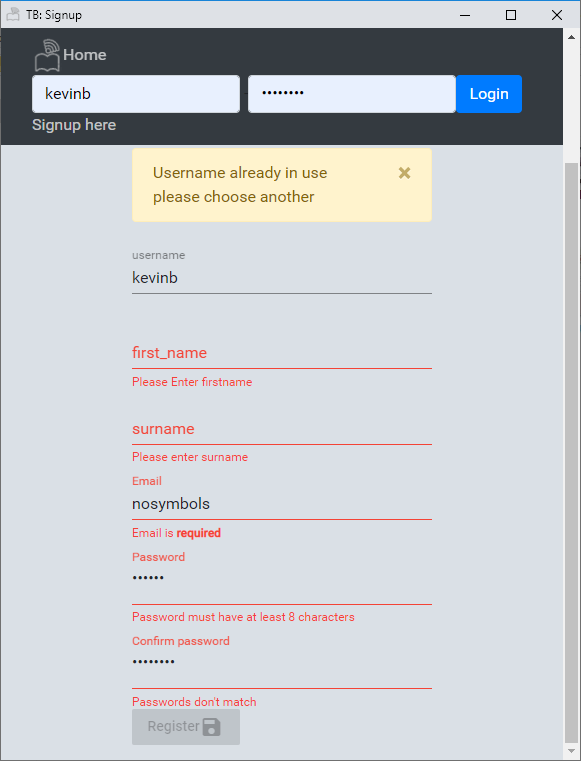
\includegraphics[width=.9\linewidth]{img/ui/signuperror.PNG} %the image must be resized or scaled if needed
\caption{Register Validation}
\end{minipage}
\end{figure}

\begin{figure}[H]
\centering
\begin{minipage}{.75\textwidth}
  \centering
  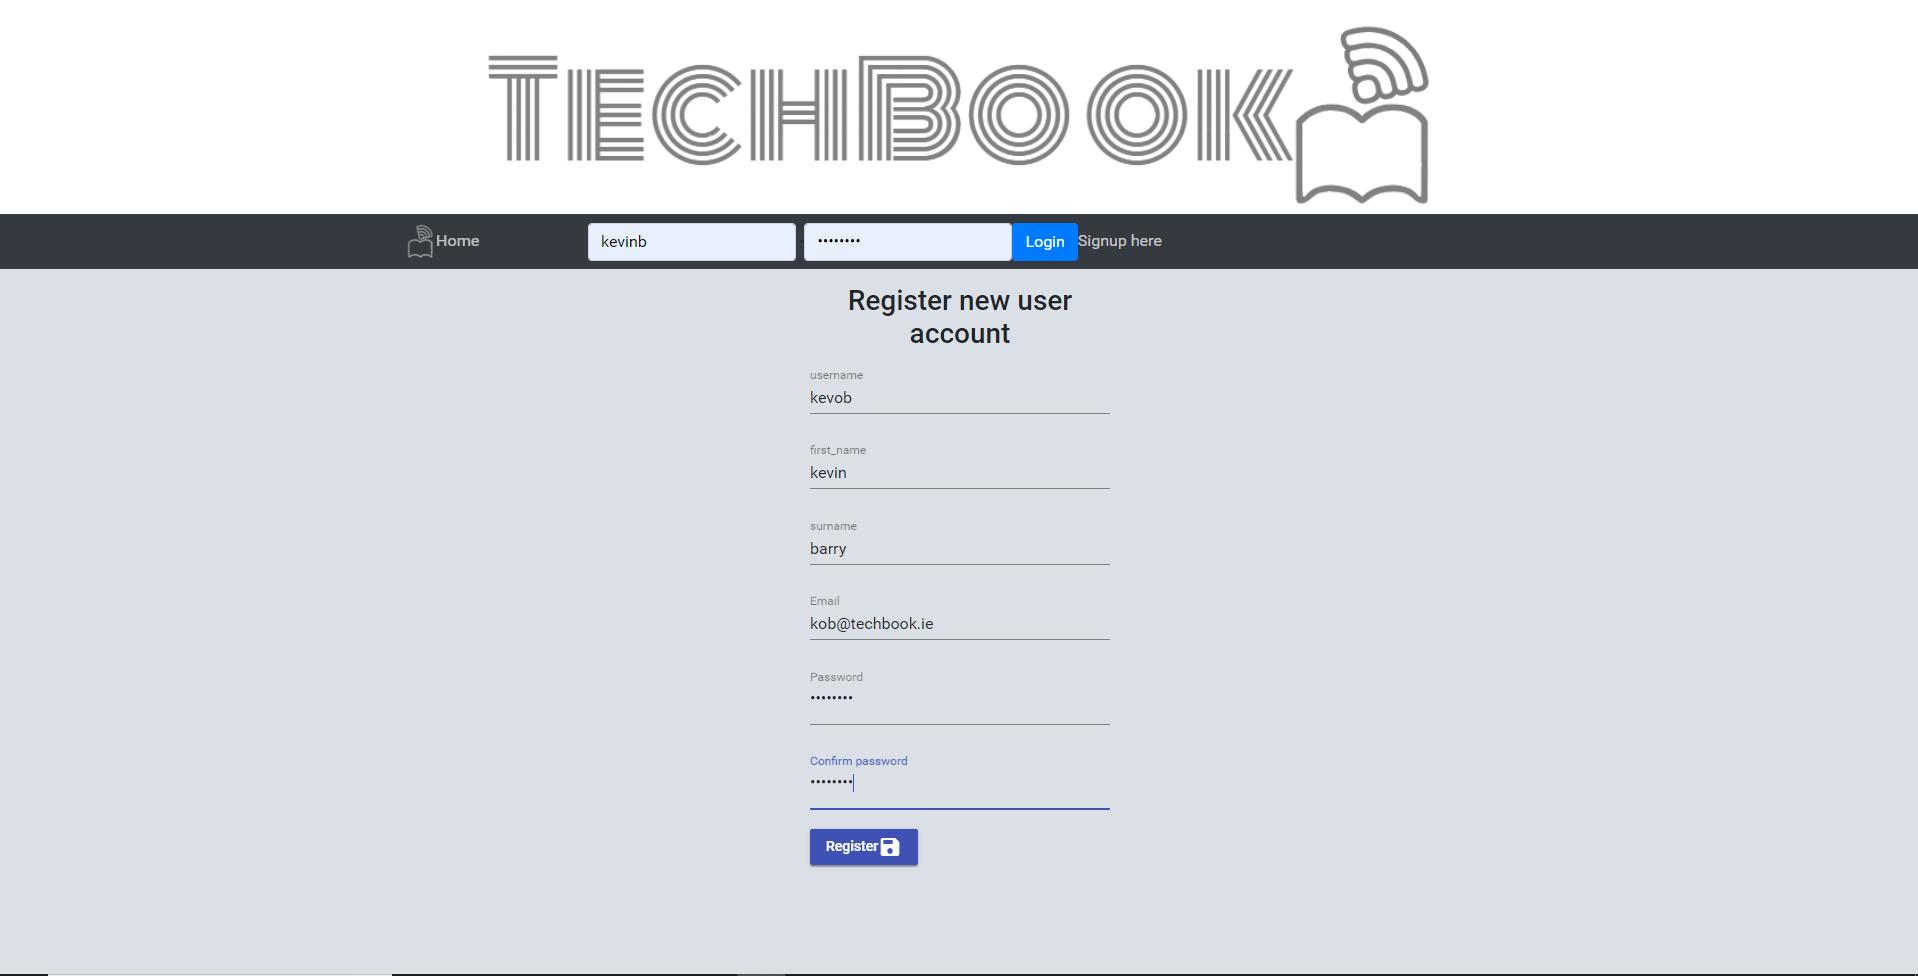
\includegraphics[width=.9\linewidth]{img/ui/sigup_PC.PNG}
  \captionof{figure}{Web View}
  \label{fig:signupPC}
\end{minipage}%
\begin{minipage}{.25\textwidth}
  \centering
  
\includegraphics[width=.9\linewidth]{img/ui/signup_MOBILE.PNG}
  \captionof{figure}{Mobile view}
  \label{fig:signupMOBILE}
\end{minipage}
\end{figure}

\subsubsection{Profile Page}
\begin{figure}[H]
\centering
\begin{minipage}{.75\textwidth}
  \centering
  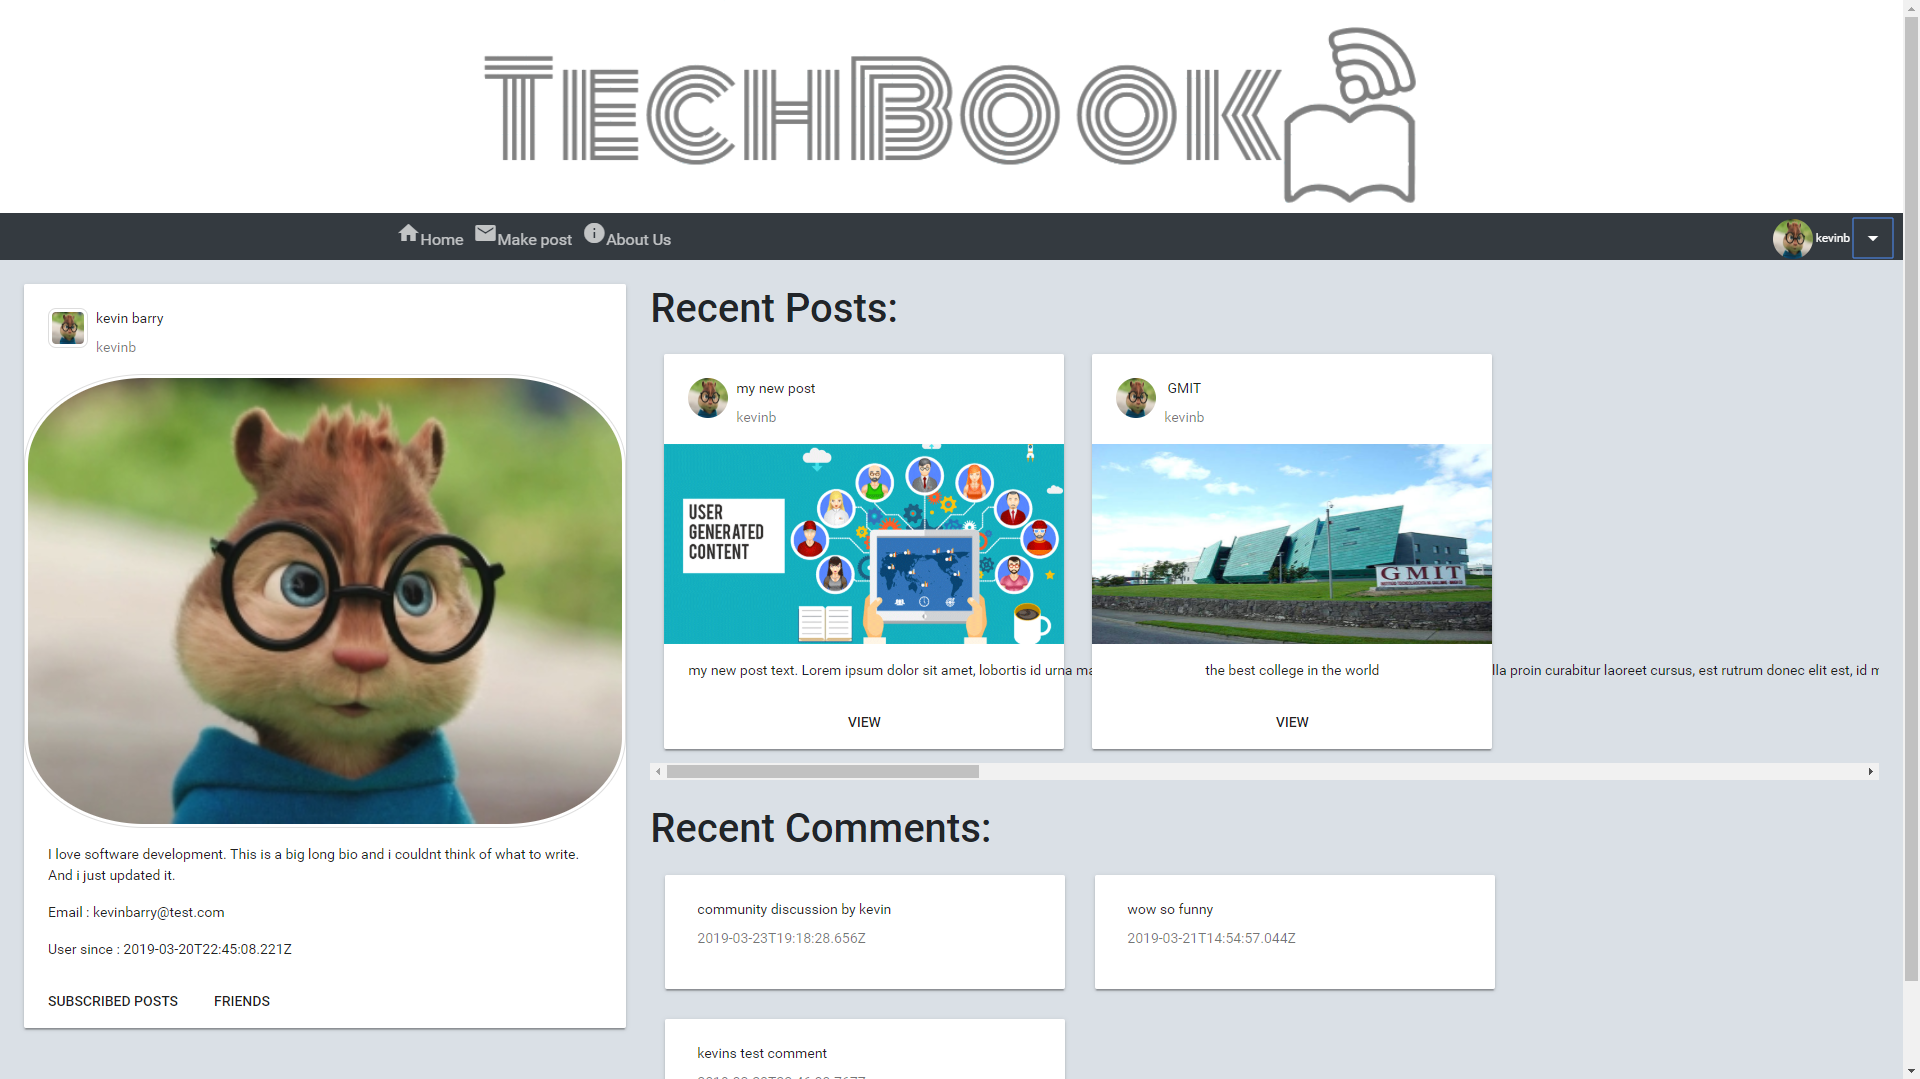
\includegraphics[width=.9\linewidth]{img/ui/profile_PC.PNG}
  \captionof{figure}{Web View}
  \label{fig:profilePC}
\end{minipage}%
\begin{minipage}{.25\textwidth}
  \centering
  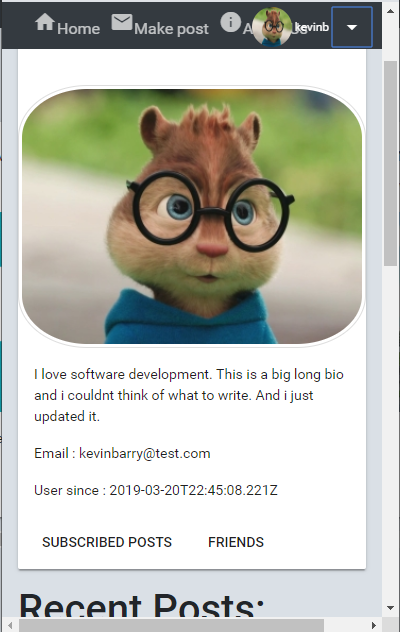
\includegraphics[width=.9\linewidth]{img/ui/profile_MOBILE.PNG}
  \captionof{figure}{Mobile view}
  \label{fig:profileMOBILE}
\end{minipage}
\end{figure}

\subsubsection{Settings Page}
The settings page view allows a user to edit their current credentials and is accessed by clicking the settings tab on the navbar drop down menu. The form fields are prefilled from the users data retrieved by the server.

\begin{lstlisting}[language=JavaScript,caption={Defining User Schema},captionpos=b,label={fig:userscema}]
/**
 * Set the form data in SettingsForm to the details of the current user.
 * 
 * @param id The current users id.
 */
setForm(id) {
  this.userService.getProfile(id)
    .subscribe(profile => {
      // Must extract profile data from response.
      this.profileinfo = profile[0];
      // Form object
      this.settingsForm.setValue({
        email: this.profileinfo.email,
        first_name: this.profileinfo.first_name,
        surname: this.profileinfo.surname,
        bio: this.profileinfo.bio
      });
    });
}
\end{lstlisting}
 This page also allows the user to update or change their current profile image. Selecting the 'choose file' button pops up a file explorer window and allows the user to select an image. The chosen image is then shown in a preview tab so the user can have a peek prior to selecting the "Upload new profile image" button. This was achieved by importing the \textbf{ng2-file-upload} module and applying custom functions. The uploaded image is then saved in a image folder on the server and the users account is updated with the location to access this image. The uploader is also validated to only accept image files.
\begin{figure}[H]
\centering
\begin{minipage}{.75\textwidth}
  \centering
  
\includegraphics[width=.9\linewidth]{img/ui/settings_PC.PNG}
  \captionof{figure}{Web View}
  \label{fig:settingsPC}
\end{minipage}%
\begin{minipage}{.25\textwidth}
  \centering
  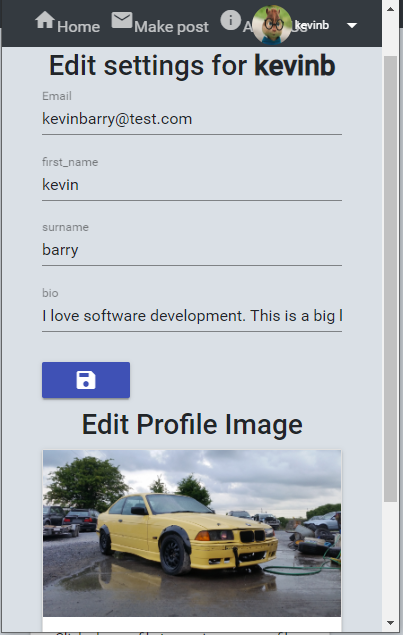
\includegraphics[width=.9\linewidth]{img/ui/settings_MOBILE.PNG}
  \captionof{figure}{Mobile view}
  \label{fig:settingsMOBILE}
\end{minipage}
\end{figure}

\subsubsection{Friends Page} 
The friends page is a view that allows a user to toggle a view between followers and following. This page can be accessed in two ways which render different views. If a user wants to view a list of their own followers and who they are following they can select the "Friends" button in the navbar drop down menu. If a user would like to view another users followers and following list a button "Follows" can be selected on the preferred users profile page. The lists contain cards that show a image avatar, username and bio for each user. To view a users profile from this view simply click on the username and the system redirects you to that users profile page.
\begin{figure}[H]
\centering
\begin{minipage}{.75\textwidth}
  \centering
  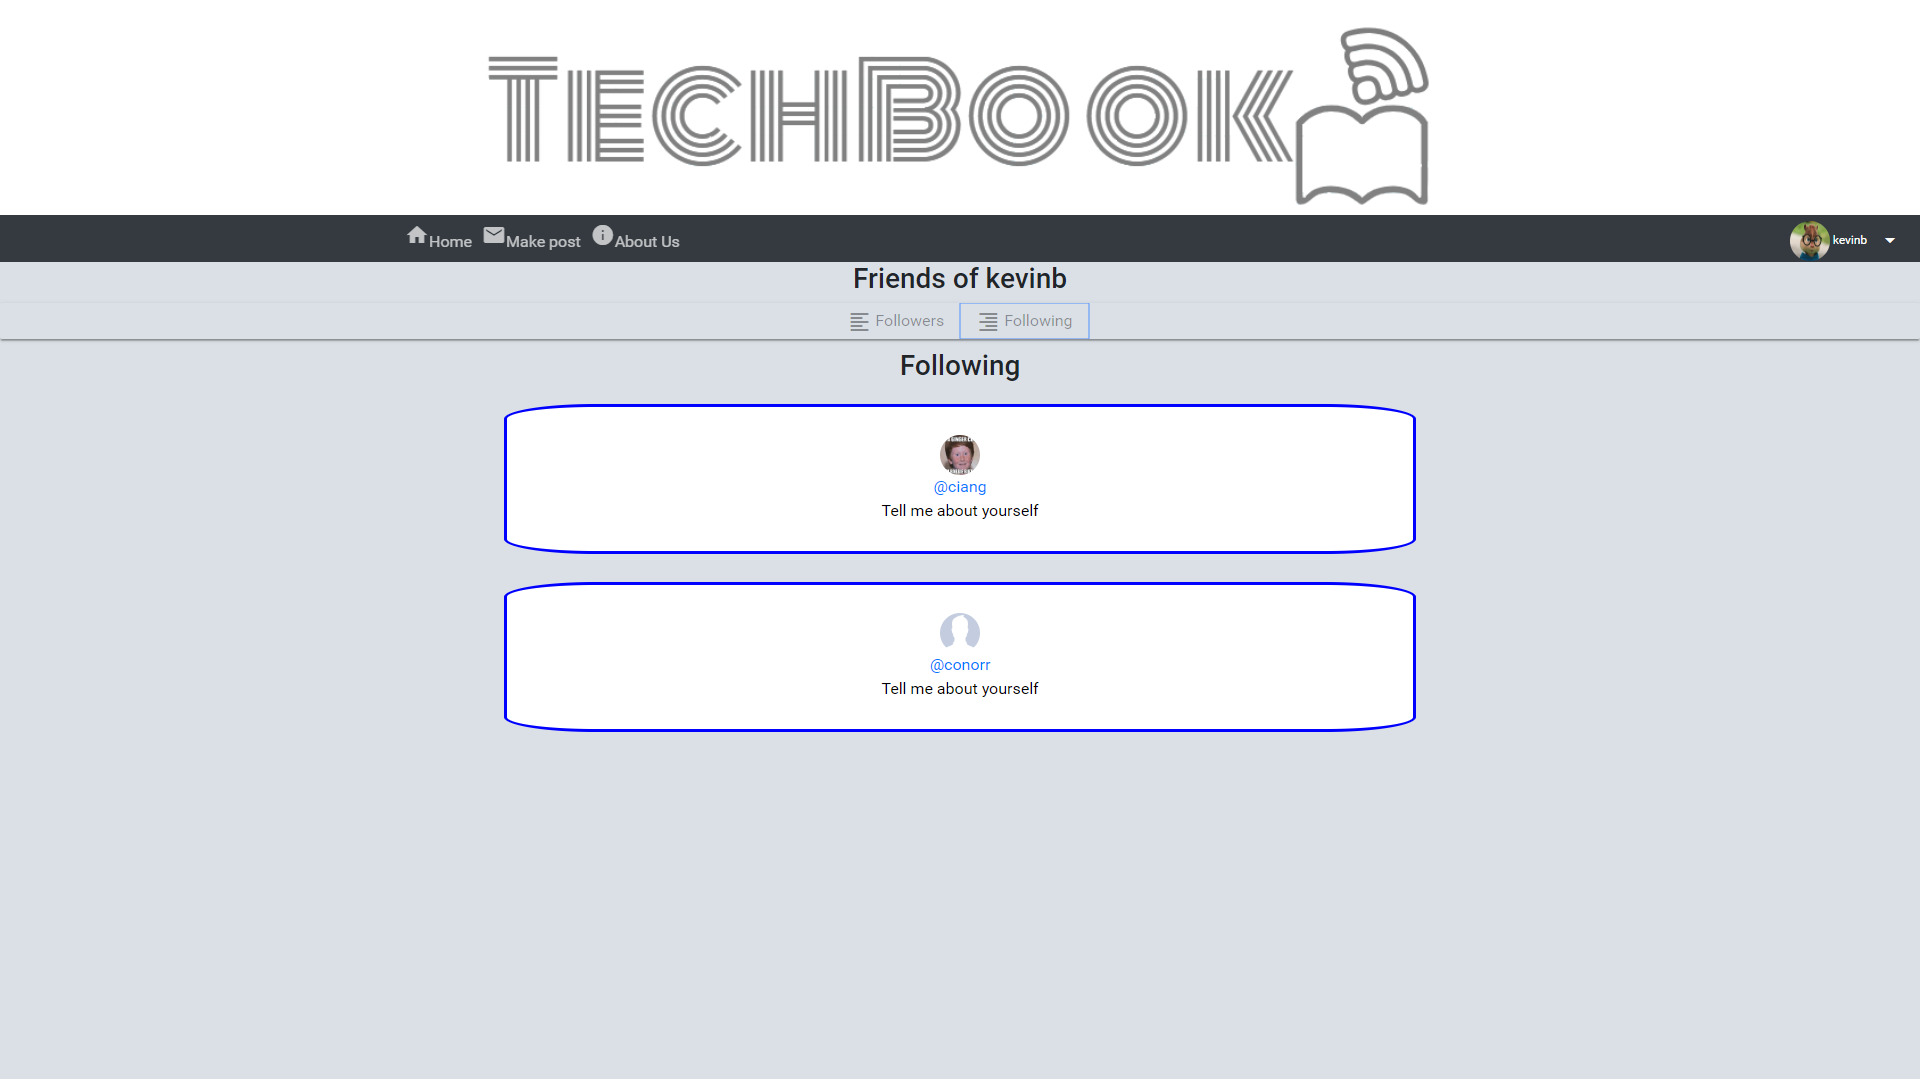
\includegraphics[width=.9\linewidth]{img/ui/followPC.PNG}
  \captionof{figure}{Web View}
  \label{fig:followPC}
\end{minipage}%
\begin{minipage}{.25\textwidth}
  \centering
  
\includegraphics[width=.9\linewidth]{img/ui/followMOBILE.PNG}
  \captionof{figure}{Mobile view}
  \label{fig:followMOBILE}
\end{minipage}
\end{figure}

\subsubsection{Home Page}

\begin{figure}[H]
\centering
\begin{minipage}{.75\textwidth}
  \centering
  
\includegraphics[width=.9\linewidth]{img/ui/homepcsnap.PNG}
  \captionof{figure}{Web View}
  \label{fig:test1}
\end{minipage}%
\begin{minipage}{.25\textwidth}
  \centering
  
\includegraphics[width=.9\linewidth]{img/ui/homemobile.PNG}
  \captionof{figure}{Mobile view}
  \label{fig:test2}
\end{minipage}
\end{figure}

\subsubsection{Posts Page}
\subsubsection{About Page}
\begin{figure}[H]
\centering
\begin{minipage}{.75\textwidth}
  \centering
  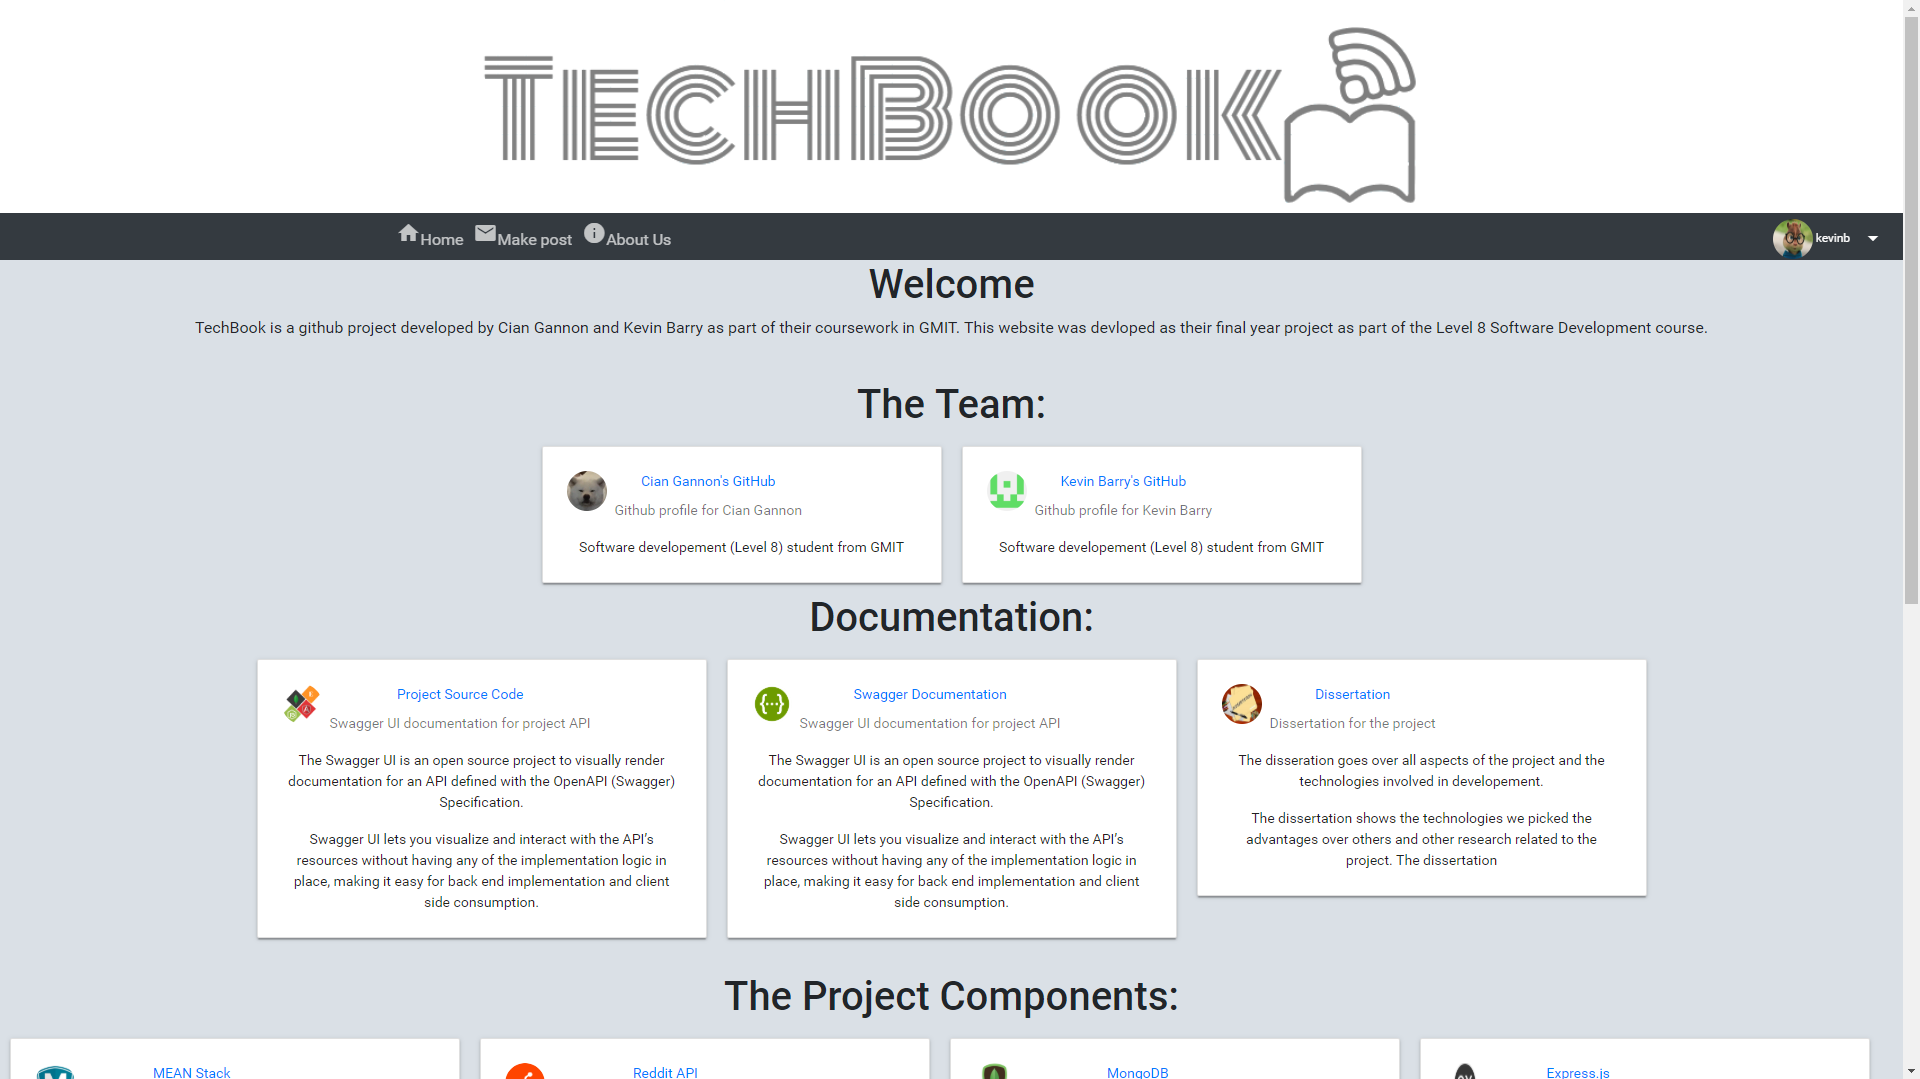
\includegraphics[width=.9\linewidth]{img/ui/about_PC.PNG}
  \captionof{figure}{Web View}
  \label{fig:aboutPC}
\end{minipage}%
\begin{minipage}{.25\textwidth}
  \centering
  
\includegraphics[width=.9\linewidth]{img/ui/about_MOBILE.PNG}
  \captionof{figure}{Mobile view}
  \label{fig:aboutMobile}
\end{minipage}
\end{figure}
\begin{itemize}
\item Architecture, UML etc. An overview of the different components of the system. Diagrams etc… Screen shots etc.
\end{itemize}

\begin{table}[h]
  \centering
  \begin{tabular}{x{2cm}p{3cm}}
    \toprule \\
    Column 1 & Column 2 \\
    \midrule \\
    Rows 2.1 & Row 2.2 \\
    \bottomrule
  \end{tabular}
  \caption{A table.}
  \label{table:mytable}
\end{table}
\chapter{System Evaluation}
Reflecting on the objectives discussed in \textit{1.1: ProjectObjectives} ,the following is a condensed initial list of objectives for both the dissertation and applied aspects this project: 

\paragraph{Dissertation}
\begin{itemize}
\item Introduce the concept of the project. 
\item Provide an understanding of social media.
\item Provide a understanding of web technologies.
\item Describe the development of the applied project
\end{itemize}
 
 \paragraph{Applied Project}
\begin{itemize}
\item Produce a simple easy to use web application.
\item Deliver a social platform for tech savvy people that differs from the norm.
\item Dive into new web technologies.
\item Complete the project collaborating as a team using an efficient and effective approach.
\end{itemize}

% ========================== Testing ========================== 
\section{Testing}
is it robust?
what type of testing?
 Prove that your software is robust. How? Testing etc. 
\subsection{Unit Testing}
testing parts of program
\subsection{Beta Testing}
giving the program to peers

% ========================== Performance ========================== 
\section{Performance}
Use performance benchmarks (space and time) if algorithmic.

% ========================== Objectives ========================== 
\section{Evaluation of Objectives}
Measure the outcomes / outputs of your system / software against the objectives from the Introduction.
\subsection{Objective 1}
did we reach our objective?

\subsection{Objective 2}
did we reach our objective?

\subsection{Objective 3}
did we reach our objective?

\subsection{Objective 4}
did we reach our objective?

% ========================== Limitations ========================== 
\section{Limitations}
Areas for improvement?
Highlight any limitations or opportuni-ties in your approach or technologies used.
\chapter{Conclusion}
About three pages.

\begin{itemize}
\item Briefly summarise your context and ob-jectives (a few lines).did we achieve our objectives on a dissertation and applied level.
\item Highlight your findings from the evalua-tion section / chapter and any opportuni-ties identified.
\item Learning outcomes achieved?
\end{itemize}

\chapter{Appendices}

\textbf{Github Organisation: }\\ \noindent\textcolor{NavyBlue}{\url{https://github.com/Final-Year-Project-Cian-Kevin}}\\

\noindent\textbf{Github Project Source Code: }\\\ \noindent\textcolor{NavyBlue}{\url{https://github.com/Final-Year-Project-Cian-Kevin/final-project}}\\

\noindent\textbf{Deployed Application Link: }\\\ \noindent\textcolor{NavyBlue}{\url{http://34.243.30.50:3000}}\\

\noindent\textbf{Swagger: }\\\ \noindent\textcolor{NavyBlue}{\url{http://34.243.30.50:3000/api-docs/}}\\

\noindent\textbf{TypeDoc: }\\\ \noindent\textcolor{NavyBlue}{\url{http://34.243.30.50:3000/typedoc/}}\\

\noindent\textbf{Video Presentation: }\\ \noindent\textcolor{NavyBlue}{\url{https://www.youtube.com/watch?v=mqdhf0jrF9I}}







